% Sección 4. Cifras: documentos/informe_resultados.md (secciones 1, 3, 4, 5 y 6; tablas 1, 1b, 1c, 2, 3, 7b, 8 y 9),
% app/DATOS.md (claves demanda_*, modelo_*, resultado_*, despacho_*, ciudad_* y piloto_*) y los README de
% E1, E11, E12, E13, E7, D5, D6, costos/, sistema_tiempo_real/ y P2 donde se indica.
\section{Resultados}
\label{sec:resultados}

Los resultados de pronóstico son de los doce pliegues mensuales de 2025 con antelación de siete días (18.615
franjas), salvo que se diga otra cosa; los de decisión evalúan cada día de 2025 con la demanda que de verdad llegó.

\subsection{Pronóstico de la demanda}
\label{sec:res-pronostico}

\paragraph{Precisión.} La regla manual de Sobusa se equivoca en 20 de cada 100 pasajeros; el modelo final, en 14
(tabla~\ref{tab:wape}). Frente al primer LightGBM (E1), el modelo final gana 0,46 puntos y mejora en 10 de 12 meses; el
híbrido con Chronos-2 gana otros 0,32 y mejora en 11 de 12. La antelación casi no cuesta: a 7, 14, 21 y 28 días el
modelo final da 13,9, 14,1, 14,3 y 14,4~\% y la regla 20,0, 20,5, 20,9 y 21,2~\%. El error del total diario por ruta baja
de 12,75~\% con la regla a 4,86~\%. Por ruta, el modelo final se equivoca un 11,54~\% en CRA~54, la más cargada, un
15,52~\% en SILENCIO y un 19,08~\% en CL~72 (la regla: 17,97, 21,51 y 24,32~\%). Por tipo de día, 13,36~\% en laborales,
13,45~\% en sábados y 19,74~\% en domingos y festivos, frente a 17,62, 15,10 y 48,58~\% de la regla: en los 17 festivos de
2025, E1 se equivoca un 25,0~\% y la regla un 145,8~\%, porque promedia ocho semanas sin el festivo. La tarde (16--20~h)
es la franja más difícil (18,35~\%). El híbrido mejora al modelo final en todas las rutas, tipos de día y franjas.

\begin{table}[t]
  \centering\footnotesize
  \setlength{\tabcolsep}{3.5pt}
  \caption{Error del pronóstico de pasajeros por ruta, día y hora de salida a una semana. WAPE en \%; diferencias
  en puntos de WAPE con IC del 95~\% por \emph{bootstrap} pareado de días.}
  \label{tab:wape}
  \begin{tabular}{@{}l r r l r r@{}}
    \toprule
    Método & WAPE 2025 & Diferencia [IC 95~\%] & Frente a & Meses mejor & WAPE 2024 \\
    \midrule
    B1: regla manual & 20,04 & $+5{,}65$ [$4{,}38$; $7{,}24$] & E1 & -- & -- \\
    E1: primer LightGBM & 14,40 & -- & -- & -- & -- \\
    Modelo final (E11, V4) & 13,94 & $-0{,}46$ [$-0{,}60$; $-0{,}33$] & E1 & 10/12 & 15,73 \\
    \textbf{Híbrido con Chronos-2 (E12)} & \textbf{13,62} & $-0{,}32$ [$-0{,}43$; $-0{,}22$] & final & 11/12 & 15,40 \\
    \bottomrule
  \end{tabular}
  \fuente{E11 y E12 (\texttt{informe\_resultados.md}, tablas 1 y 1b; por segmento, \texttt{app/DATOS.md}:
  \texttt{demanda\_wape\_por\_ruta}, \texttt{\_por\_tipo\_dia} y \texttt{\_por\_franja}). En 2024, fuera de la muestra de
  selección, el híbrido mejora al modelo final en $-0{,}33$ [$-0{,}50$; $-0{,}14$] puntos y en 10 de 12 meses.}
\end{table}

\paragraph{Qué aporta cada componente.} En la ablación (sección~\ref{sec:ablacion}; figura~\ref{fig:ablacion}), lo
único que mejora con significancia es no aprender de los datos corruptos: los pesos de muestra ganan 0,38 puntos
[0,26; 0,50] y mejoran 10 de 12 meses; la ganancia del modelo final frente a E1 se concentra en agosto de 2025 (sin ese
mes, 0,21 puntos). Los calendarios escolar y universitario ($-0{,}05$ [$-0{,}13$; $+0{,}03$]), la climatología
($-0{,}08$ [$-0{,}15$; $0{,}00$]) y la corrección de rezagos no son significativos; la recencia empeora ($+0{,}05$
[$+0{,}005$; $+0{,}09$]) y la lluvia observada del mismo día no cambia nada. Un modelo por ruta no supera al conjunto
($-0{,}14$ puntos de media mensual, $p = 0{,}36$): el 95,1~\% de los desvíos de las rutas es un choque común. La mejor
combinación de la búsqueda aleatoria de hiperparámetros daba 13,43~\% en sus cuatro pliegues y 14,50~\% en los doce,
peor que C0 (14,40~\%), y el ajuste anidado empeora 0,07 puntos [0,02; 0,13]: el modelo final usa C0. Lo que más pesa es
la media de las cuatro semanas anteriores (57,5~\% de la ganancia) y la propia regla manual (26,7~\%).

\begin{figure}[t]
  \centering
  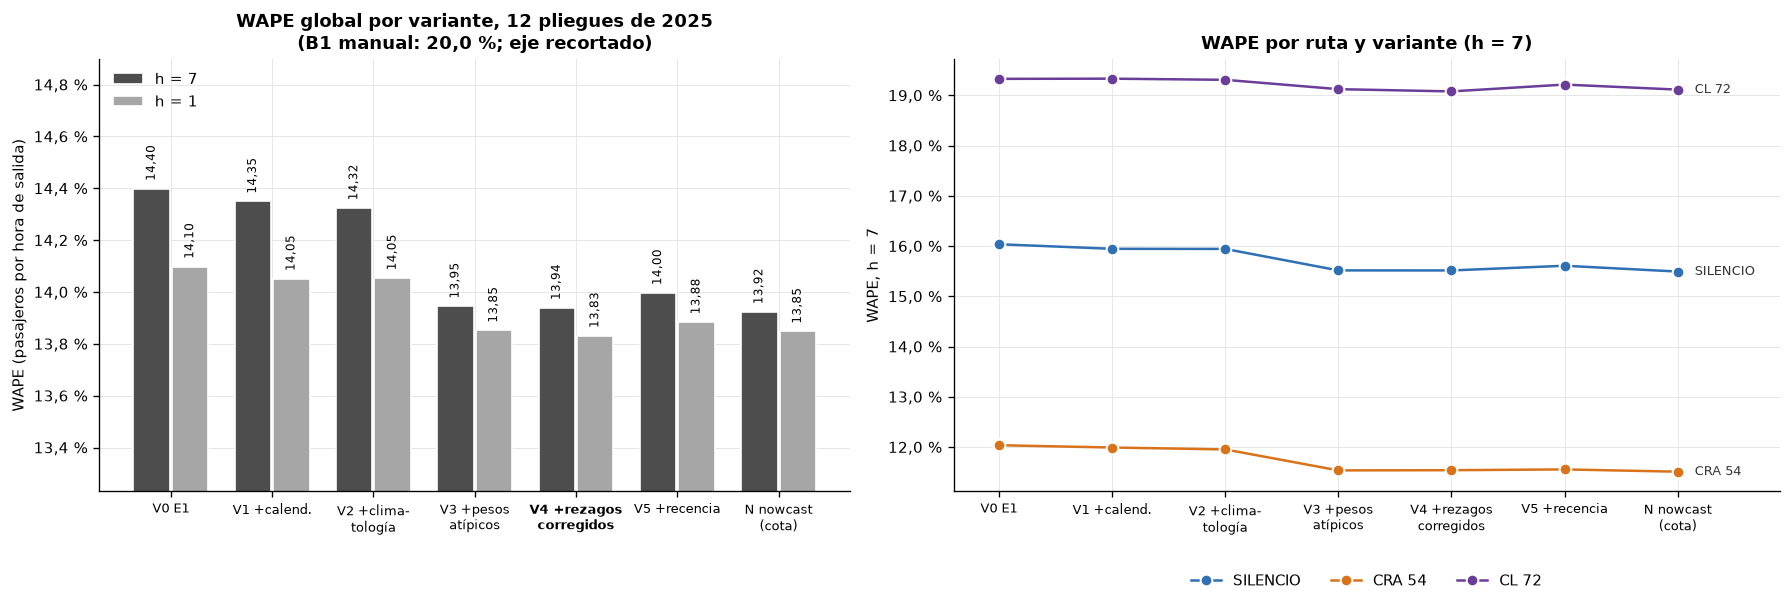
\includegraphics[width=0.78\linewidth]{e11_wape_variantes_ruta.png}
  \caption{Estudio de ablación. Izquierda: WAPE de cada variante con antelación de 7 y de 1 día (el modelo final es
  V4). Derecha: WAPE por ruta con $H = 7$.}
  \fuente{E11, \texttt{fig1\_wape\_variantes\_ruta.png}.}
  \label{fig:ablacion}
\end{figure}

\paragraph{Comparación de 51 modelos (E12).} Con el mismo protocolo, ningún modelo solo supera al LightGBM final
(tabla~\ref{tab:e12}): los otros árboles empatan, la mejor red (Temporal Fusion Transformer) queda 0,26 puntos peor y los
fundacionales sin reentrenar necesitan el calendario local (sin él quedan entre 17,1 y 18,4~\%, porque pronostican casi
el doble en los festivos). La ganancia viene de combinar modelos que se equivocan distinto. Doce candidatos cumplen la
regla de selección y el ganador formal es un apilamiento de 40 modelos, pero no se pudo repetir en 2024, y uno parecido de
seis modelos no se sostuvo ahí ($-0{,}23$ [$-0{,}49$; $+0{,}09$]). Por eso se recomienda el híbrido: el mismo LightGBM con
cuatro columnas más (el pronóstico de Chronos-2 con calendario), la única mejora confirmada fuera de la muestra de
selección con un costo casi igual. Sobrevive a Holm ($p = 0{,}002$) y, simulando su uso con 11 orígenes de fin de mes, se
equivoca un 13,70~\% frente a 13,99~\% ($-0{,}30$ [$-0{,}45$; $-0{,}15$]). Chronos-2 no se reentrena ni necesita GPU: unos
4 minutos de CPU por semana.

\begin{table}[t]
  \centering\footnotesize
  \setlength{\tabcolsep}{2.4pt}
  \caption{Mejores candidatos de cada familia y combinaciones frente al modelo final (WAPE a una semana).}
  \label{tab:e12}
  \begin{tabular}{@{}l r r r r@{}}
    \toprule
    Candidato & WAPE 2025 & Dif. [IC 95~\%] & Meses mejor & Dif. 2024 [IC 95~\%] \\
    \midrule
    TimesFM 2.5 con calendario & 14,96 & $+1{,}02$ [$0{,}67$; $1{,}43$] & 0/12 & $+0{,}72$ \\
    Chronos-2 con calendario & 14,71 & $+0{,}77$ [$0{,}47$; $1{,}14$] & 2/12 & -- \\
    Mejor clásico (AutoETS) & 14,62 & $+0{,}68$ [$0{,}38$; $1{,}04$] & 2/12 & -- \\
    Mejor red (TFT) & 14,19 & $+0{,}26$ [$0{,}01$; $0{,}50$] & 5/12 & -- \\
    XGBoost, CatBoost, LightGBM Tweedie & 13,91--14,01 & dentro del ruido & -- & -- \\
    Modelo final (E11) & 13,94 & -- & -- & (15,73) \\
    Media de 5 árboles de \emph{boosting} & 13,76 & $-0{,}18$ [$-0{,}23$; $-0{,}12$] & 11/12 & -- \\
    \textbf{Híbrido con Chronos-2} & \textbf{13,62} & $-0{,}32$ [$-0{,}43$; $-0{,}22$] & 11/12 & $-0{,}33$ [$-0{,}50$; $-0{,}14$] \\
    Media del final y los mejores de familia & 13,59 & $-0{,}35$ [$-0{,}48$; $-0{,}21$] & 12/12 & $-0{,}49$ [$-0{,}71$; $-0{,}26$] \\
    Apilamiento de 40 (ganador formal) & 13,39 & $-0{,}55$ [$-0{,}69$; $-0{,}41$] & 12/12 & no probado \\
    \bottomrule
  \end{tabular}
  \fuente{E12 (\texttt{informe\_resultados.md}, tabla 1b). Fundacionales sin reentrenar. La figura
  \texttt{fig1\_ranking\_wape\_ic.png} de E12 muestra los 24 mejores con sus intervalos.}
\end{table}

\paragraph{Pronosticar lo que de verdad sube (E13) y 2026.} Contra el objetivo corregido, el modelo final tiene un WAPE
de 13,55~\%; reentrenado con ese objetivo, 11,77~\%, y el híbrido reentrenado, 11,38~\%. Casi todo es nivel: reentrenar
gana 0,31 puntos [0,20; 0,42] y el híbrido añade 0,39. Con el objetivo viejo el plan queda corto de buses en el 44~\% de
las horas; con el corregido, en el 27--28~\%. En 2026, el modelo de largo plazo de E8, que había pronosticado 2025 con un
1,4~\% de error, se quedó un 14,6~\% corto entre el 1 de enero y el 10 de agosto, en las 21 combinaciones de ruta y día
de la semana: un error de nivel, no de forma. Según los agregados de Sobusa, los viajes crecieron un 14,6~\% y las subidas
un 7,5~\% frente a 2025. Falta confirmarlo con los viajes de 2026; si es real, el modelo final y el híbrido, que
pronostican para las primeras semanas de 2026 entre un 11 y un 14~\% menos que 2025, quedarían cortos: hay que
reentrenar cada semana.

\subsection{Decisión de despacho}
\label{sec:res-decision}

\paragraph{La demanda responde a la oferta.} La elasticidad por hora es 0,73 (IC 0,70--0,75; $F = 2.177$ en la primera
etapa); por ruta-día, 0,66 (0,54--0,78), y el derrame indica 0,80--0,90: de los 83,8 pasajeros esperados en un viaje
que falla, los cuatro buses siguientes recogen solo el 16,8~\%. La síntesis es $\beta \approx 0{,}70$ (0,55--0,90), por
encima del 0,5 de la literatura (0,67 en SILENCIO, 0,66 en CRA~54 y 0,80 en CL~72). Sobusa pierde más que el promedio,
probablemente porque compite en corredores compartidos. La definición ingenua, con la marca \texttt{cancelada}, da 1,02
por pura construcción.

% Plan que recorta: +1.939 M (simétrica), -1.512 pasajeros netos, 530 sobre la capacidad y 4,74 min de espera, de
% costos/resultados/d5_reoptimizado.csv (corrida «D5 original»). Neto con beta = 0,90: -2.140, exacto, de
% simulacion_ahorro/resultados/sensibilidad_beta.csv (plan a); el tornado de costos/ da -2.137 porque interpola la
% curva A(1 - c^beta) (costos/resultados/validacion_interpolacion_beta.csv). 562 bajadas forzadas por día laboral:
% experimentos/D6_simulador/escenarios_resumen.csv (CRA 54, S0+G).
\paragraph{Recortar no paga con la contabilidad conservadora.} El optimizador con los supuestos iniciales recortaba el
9,6~\% de las horas de bus (60.754 al año) y 1,05 millones de km (tabla~\ref{tab:escenarios}). Con costos con fuente,
ese recorte ahorra 3.695 M COP al año en operación pero pierde 4.724 M en pasajes con $\beta = 0{,}70$: un neto de
$-1.029$ M ($+1.939$ M con la simétrica, pero con 1.512 pasajeros netos menos al día). Deja de pagar con
$\beta > 0{,}53$ (con los supuestos, en 0,85); la regla fija S1 pierde 1.713 M y su equilibrio, 0,36, queda por debajo
de todas las mediciones. Solo son positivos el optimizador con intervalo máximo de 15 minutos (+390 M COP) y el giro
corto en el punto 35 de CRA~54 (+248 M), que obliga a bajarse antes a 562 pasajeros por día laboral. $\beta$ mueve el
neto del plan que recorta de $-133$ a $-2.140$ M COP al año y el precio del ACPM apenas de $-1.058$ a $-978$: el signo depende de
$\beta$ y de cómo se cuentan los pasajeros, no de los precios. Simulado fecha por fecha, solo paga recortar domingos y
festivos (+181 M COP al año), con unos 3.810 pasajeros en riesgo por día.

\begin{table}[t]
  \centering\footnotesize
  \setlength{\tabcolsep}{4pt}
  \caption{Escenarios de 2025, tres rutas, promedio por día. Neto con costos con fuente, $\beta = 0{,}70$, conductor
  pagado por hora y contabilidad conservadora.}
  \label{tab:escenarios}
  \begin{tabular}{@{}l r r r r r r r@{}}
    \toprule
    Escenario & Salidas & Buses-hora & Espera & Sobre cap. & FC $> 1$ & Neto (M COP/año) & $\beta$ equil. \\
    \midrule
    S0 oferta real & 460 & 1.732 & 4,43 & 317 & 11,7~\% & -- & -- \\
    S1 regla D1 (máx. 10 min) & 431 & 1.645 & 4,51 & 384 & 9,9~\% & $-1.713$ & 0,36 \\
    S5 regla D1 (máx. 15 min) & 407 & 1.555 & 4,87 & 422 & 12,4~\% & $-409$ & 0,63 \\
    D5 con supuestos & 411 & 1.565 & 4,74 & 530 & 15,6~\% & $-1.029$ & 0,53 \\
    D5 con máx. 15 min & 384 & 1.460 & 5,19 & 593 & 19,6~\% & $+390$ & 0,76 \\
    D5 con penalidad 30.000 & 447 & 1.702 & 4,36 & 264 & 7,1~\% & $-2.462$ & 0,17 \\
    \textbf{D5 con costos con fuente} & \textbf{451} & \textbf{1.723} & \textbf{4,30} & \textbf{267} & \textbf{6,8~\%} & $\bm{-2.825}$ & -- \\
    \bottomrule
  \end{tabular}
  \fuente{D5 y \texttt{costos/} (\texttt{informe\_resultados.md}, tabla 3). Espera media en minutos; sobre cap.:
  pasajeros por día por encima de 50 a bordo; FC $> 1$: horas con factor de carga mayor que 1. Con la contabilidad
  simétrica, el plan que recorta deja +1.939 M COP al año y el que reasigna, +1.600.}
\end{table}

\paragraph{Con costos con fuente, el óptimo reasigna.} Reoptimizado con los costos con fuente
(sección~\ref{sec:decision}), el optimizador ya no recorta: 451 salidas al día frente a 460, con casi las mismas horas
de bus ($-0{,}5$~\%), menos espera (de 4,43 a 4,30 minutos) y menos sobrecarga (de 317 a 267 pasajeros diarios sobre la
capacidad). Quita salidas en los valles de CRA~54, en SILENCIO y en domingos y festivos, y las pasa a CL~72 (de 81 a 104
salidas al día) y a la franja de 13 a 15~h de los días laborales (de 88,7 a 110,2 salidas en las tres rutas;
figura~\ref{fig:reasigna}). Ahorra poco en operación (+501 M COP al año); el canje es la contabilidad: contando solo los pasajeros perdidos, el plan arriesga 2.864 al
día y su saldo es de $-2.825$ M COP al año; si los ganados cuentan igual, gana 946 pasajeros netos al día y $+1.600$ M
COP. Cuál vale lo debe medir el piloto. En caja, recortar queda mejor en las dos contabilidades, pero pierde más
pasajeros, tiene casi el doble de sobrecarga (530 frente a 267 al día) y sube la espera a 4,74 minutos; el optimizador,
que valora la espera y la sobrecarga con supuestos, prefiere reasignar. El simulador confirma en CRA~54 la sobrecarga del plan que recorta, no la espera: 12,1~\% menos
buses-hora sin cambio de espera distinguible del azar, pero con el 46~\% de los viajes a 50 a bordo, frente al 35,5~\%.
En CL~72 basta regularizar: las mismas salidas, equiespaciadas, bajan la espera de 9,5 a 8,0 minutos.

\begin{figure}[t]
  \centering
  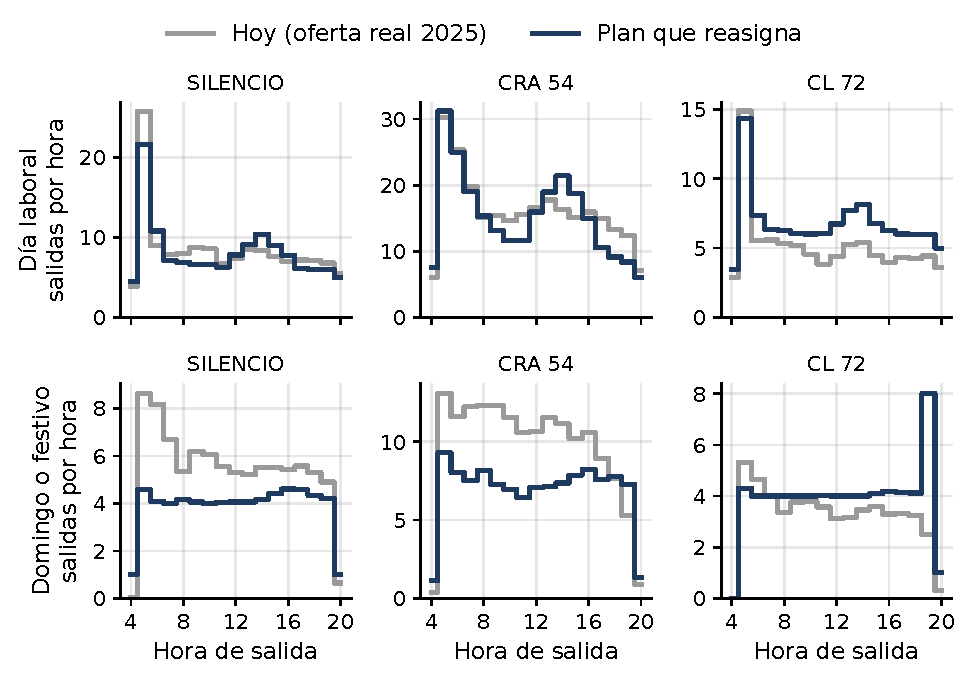
\includegraphics[width=0.62\linewidth]{fig_plan_reasigna.pdf}
  \caption{Salidas válidas por hora de salida, promedio por día de 2025: oferta real (gris) y plan que reasigna
  (azul), por ruta, en días laborales (arriba) y en domingos y festivos (abajo).}
  \fuente{elaboración propia con \texttt{costos/resultados/d5\_reoptimizado\_decisiones.parquet} (corrida \comi{D5
  costos nuevos, pago por hora, e=0,5}) y \texttt{figuras\_extra.py}.}
  \label{fig:reasigna}
\end{figure}

\subsection{Operación en tiempo real}
\label{sec:res-tiempo-real}

Corregir la demanda con lo visto en el día no aporta: el pronóstico semanal ya acierta el total del resto del día con
un 5--8~\% de error por ruta hasta el mediodía, y el ajuste calibrado deja el error por hora igual (a las 12~h, de
14,25~\% a 14,27~\%; sin calibrar, lo empeoraba a 18,3~\%). Las decisiones tampoco mejoran: el plan semanal queda a 1,05
salidas por hora del óptimo y el motor, a 1,08 (tabla~\ref{tab:oraculo}). La brecha grande está en la operación real, a
2,80: con sus mismos buses-hora ($-0{,}2$~\%), el plan da menos espera (4,99 frente a 5,16 minutos), menos sobrecarga
(68 frente a 107 pasajeros al día) y 1,7 M COP diarios menos de costo generalizado. El valor del tiempo real está en
ejecutar bien el plan: la hora exacta de cada salida, cerrar huecos, no despachar buses pegados y detectar fallas de
datos (la guarda reconoce los tres días de 2025 en que falló el registro). Falta pulir las alertas: el sobrecupo salta
en 21,7 y la regularidad en 16,9 de cada 69 corridas por ruta y día.

\begin{table}[t]
  \centering\footnotesize
  \setlength{\tabcolsep}{3.5pt}
  \caption{Decisiones frente al óptimo con la demanda que llegó: 79 días de 2025, horas 7--20, promedio diario.}
  \label{tab:oraculo}
  \begin{tabular}{@{}l r r r r@{}}
    \toprule
    Escenario & Error (salidas/h) & Horas exactas & Sobre cap./día & Costo (M COP/día) \\
    \midrule
    Plan semanal (D5, costos con fuente) & 1,05 & 53,9~\% & 68 & 86,2 \\
    Motor (plan corregido en el día) & 1,08 & 52,6~\% & 77 & 86,5 \\
    Oferta real 2025 & 2,80 & 13,9~\% & 107 & 87,9 \\
    Óptimo con la demanda que llegó & 0 & 100~\% & 7 & 81,6 \\
    \bottomrule
  \end{tabular}
  \fuente{tiempo real (\texttt{informe\_resultados.md}, tabla 9), corrida del 13 de octubre de 2026. Costo generalizado:
  operación con costos con fuente, espera a 7.000 COP por hora y sobrecarga a 10.000 COP por pasajero.}
\end{table}

\subsection{El modelo persona a persona y un hallazgo honesto}
\label{sec:res-persona}

Las cifras anteriores reparten la carga de cada hora entre sus buses; el modelo persona a persona sigue a cada pasajero
real hasta un bus concreto del plan. En los 353 días de 2025 con GPS, el plan pone 451 salidas por día frente a 491
reales (452 válidas) y ahorra 3,9 M COP de operación al día ($-3{,}8$~\%), pero pierde 4.092 pasajeros al día
(10,7~\%): 3.130 por la regla de $\beta$ y 962 que no encuentran bus del plan en 20 minutos. La espera media sube de
3,53 a 4,07 minutos y las personas por encima de la capacidad, de 388 a 2.742 al día. El saldo del año es de $-3.212$ M
COP con la contabilidad conservadora y de $+2.312$ M con la simétrica, del mismo orden que la tabla~\ref{tab:escenarios}
(estas cifras no tuvieron revisor independiente). El promedio esconde cuánto cambia el plan por tipo de día: los
domingos y festivos pierden el 29~\% de las salidas y son los únicos días que pagan con la cuenta conservadora (+5,1 M
COP por día), mientras que el saldo es negativo en 231 de 237 días laborales. El martes 3 de junio de 2025 el plan pone
507 salidas frente a 600 reales (548 válidas), y en CRA~54, de 17 a 19~h, 10, 9 y 7 donde hubo 15, 19 y 14 válidas: las
personas por encima de 50 a bordo pasan de 516 a 3.838 y se pierden 5.879 pasajeros ($-4{,}1$ M COP). Los peores días
son los de Carnaval, que el plan trata como laborales. El optimizador no lo ve porque reparte la carga de la hora entre
todos sus buses: hace falta una restricción de cupo por bus o una penalidad mayor por hacinamiento, y el piloto es
imprescindible.

\subsection{Piloto para medir \texorpdfstring{$\beta$}{beta} (P2)}
\label{sec:res-piloto}

$\beta$ se midió con fallas imprevistas, que dejan un hueco doble sin aviso; un recorte planificado y parejo podría
perder menos (0,4--0,5). Por eso diseñamos un piloto de ocho semanas en CRA~54 y CL~72 con días alternos sorteados y sin
anunciar al público (37 días laborales y 8 domingos). Se diseñó para el 19 de octubre al 13 de diciembre de 2026; si
Sobusa lo aprueba con esta entrega, la ventana siguiente es del 15 de febrero al 11 de abril de 2027, con el sorteo
rehecho para el lunes en que arranque. Las franjas son
CRA~54 laboral de 9 a 11~h (3 salidas menos por hora, de 16, 15 y 16 a 13, 12 y 13) y de 17 a 19~h (4 menos), CRA~54 de
9 a 13~h en cuatro de los ocho domingos (4 menos), CRA~54 laboral de 14 a 15~h (4 más) y CL~72 laboral de 12 a 15~h
(2 más). $\beta$ se estima con la forma de la ecuación~\eqref{eq:beta} y el sorteo como instrumento. La $\beta$ conjunta de
recorte tendría un error estándar de 0,056 (analítico) a 0,066 (simulado), suficiente para distinguir 0,70 de 0,53 con
probabilidad de 0,92 y 0,89 (figura~\ref{fig:potencia}). El piloto arriesga 22.904 pasajeros, el 0,30~\% del año de
CRA~54, con un saldo entre $-51{,}9$ y $+22{,}1$ M COP y cinco reglas de parada. Mide también si los buses añadidos
atraen pasajeros: reasignar no pierde pasajeros si la $\beta$ de refuerzo llega a 0,66, ni dinero si llega a 0,62.


\begin{figure}[t]
  \centering
  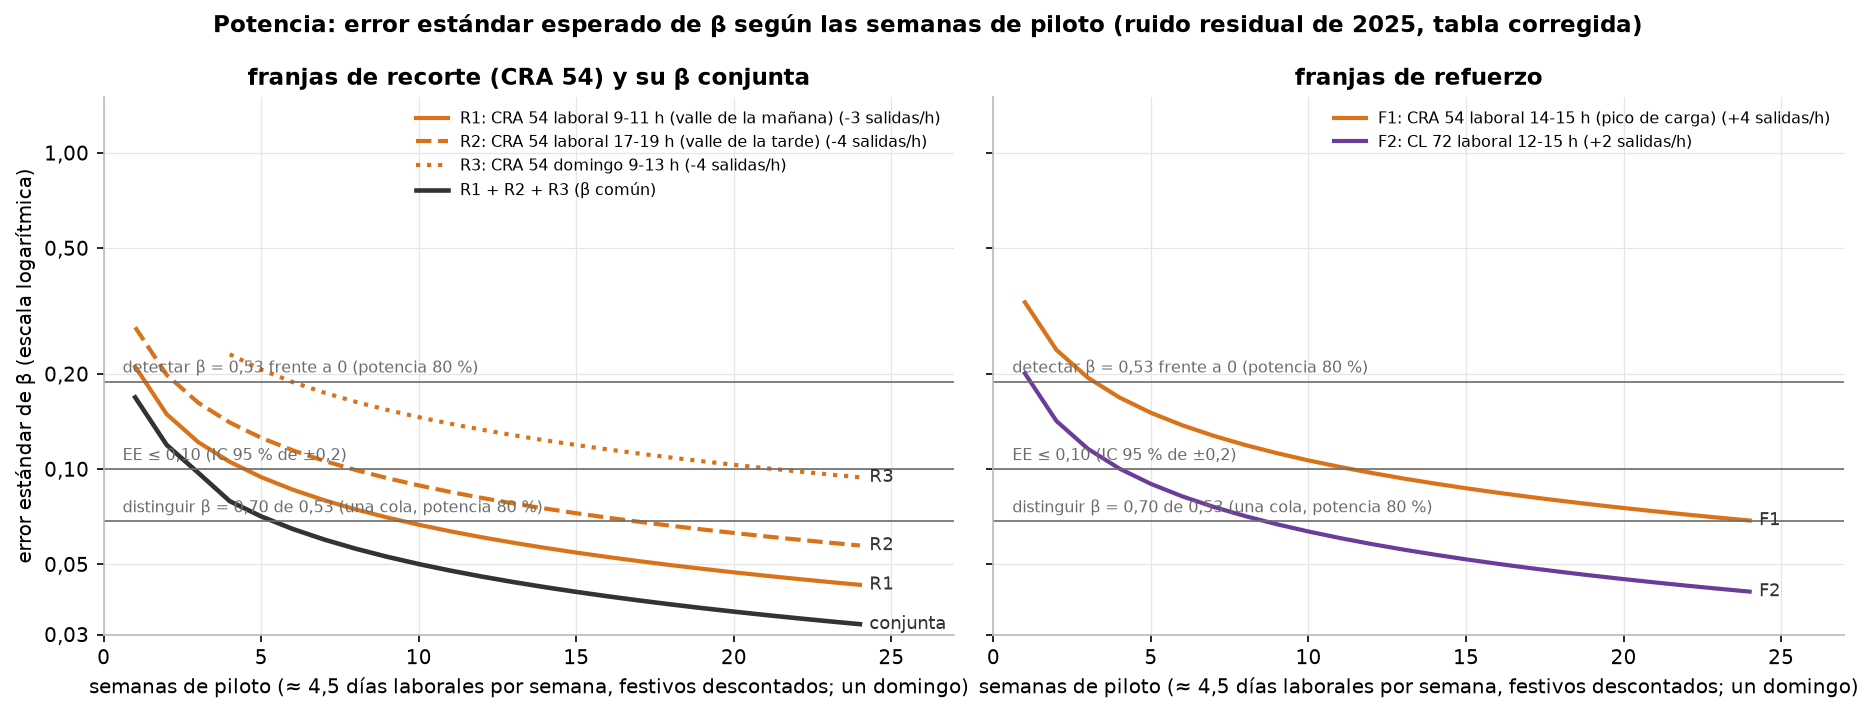
\includegraphics[width=0.6\linewidth]{p2_potencia.png}
  \caption{Error estándar esperado de $\beta$ según las semanas de piloto, para las franjas de recorte y su $\beta$
  conjunta (izquierda) y para las de refuerzo (derecha), con los umbrales de detección.}
  \fuente{P2, \texttt{fig2\_potencia.png}.}
  \label{fig:potencia}
\end{figure}
